\scanpage{75}
% archive sheet number: 76
\[
\sum_1^n\log(1+r\rho_i(u+v))\leq\sum_1^n\log(1+r\rho_i(u))+\sum_1^n\log(1+r\rho_i(v))
\]

\[
S_{\deleted{\unsure{m}}\varphi}^{n}(u+v)\leq S_\varphi^n(u)+S_\varphi^n(v)\qquad S_\varphi^n(w)=\sum_1^n f_\varphi(\rho_i(w))
\]

\[
f_\varphi(\rho)=\int_0^{+\infty}\frac{\varphi(r)}{\frac1\rho+r}\,dr=\int_0^{+\infty}\varphi\left(\frac s\rho\right)\frac{ds}{1+s}
\]

$\varphi$ fonction décroissante

(motivation : \inserted{Si $A(0)=B(0)=0$ ($=0$ est un \unsure{symbole|exemple}), alors} $A(r)\leq B(r)$ pour $0\leq r\leq+\infty$ équivaut à $\int\psi(r)A(r)\,dr\leq\int\psi(r)B(r)\,dr$ pour toute $\psi\geq0$ à support cp\textsuperscript{t} dans $[a,b]$, Or, en posant $\psi(r)=-\varphi'(r)$, $\varphi$ fonction \unsure{décroissante} \inserted{\unsure{continûment} \uline{différentiable}}, nulle en $b$ : \deleted{(\unsure{continûment} \inserted{nulle} \unsure{continue au} \illegible{1}} \unsure{(ce qui est $+\infty$)} et supposant \deleted{\unsure{de}}

que $A$ est dérivable $-\int\psi(r)A(r)\,dr=[-\varphi(r)A(r)]_0^{+\infty}+\int\varphi(r)A'(r)\,dr$ et le premier terme est nul, d'où $\int\varphi(r)A'(r)\,dr$. Si donc $A$ et $B$ sont dérivables, alors on obtient donc

\[
\int\varphi(r)A'(r)\,dr\leq\int\varphi(r)B'(r)\,dr
\]

pour toute fonction $\varphi$ continûment différentiable, décroissante \inserted{sur $[0,+\infty[$} et nulle au voisinage de $+\infty$. Si en plus $A'(r)$, $B'(r)\geq0$, alors \unsure{ça|ceci} sera vrai pour \deleted{toute} fonction décroissante \unsure{telle ou nulle|telle ou non nulle}, \unsure{pouvant|quand|pourvu} \unsure{être|bien|que} \unsure{infinie|intégrales}. (Si on prend

$\varphi=$

\figure{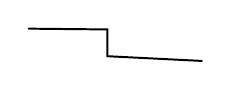
\begin{tikzpicture}[x=1mm,y=1mm,line cap=round]\draw[line width=.25mm] (0,3.5)--(10,3.4)--(10,0)--(22,-.6);\end{tikzpicture}}

, on retrouve $A(r)\leq B(r)$). Dans le cas actuel,

\[
A\deleted{\unsure{^{\,\prime}|{}^{\sim}}}(r)=\sum_1^n\log(1+r\rho_i(u))\qquad \text{donc }\ A'(r)=\sum\frac{r}{1+r\rho_i(u)}
\]

d'où notre assertion. Le cas le plus \deleted{\unsure{important}}\unsure{important} est celui où on prend $\varphi(r)=r^{-p}$ $0<p<1$. On trouve alors
